\section{mo\-HCMove\-Loop\-Expl$<$ M $>$ Class Template Reference}
\label{classmo_h_c_move_loop_expl}\index{moHCMoveLoopExpl@{moHCMoveLoopExpl}}
Iterative explorer used by a {\bf mo\-HC}{\rm (p.\,\pageref{classmo_h_c})}.  


{\tt \#include $<$mo\-HCMove\-Loop\-Expl.h$>$}

Inheritance diagram for mo\-HCMove\-Loop\-Expl$<$ M $>$::\begin{figure}[H]
\begin{center}
\leavevmode
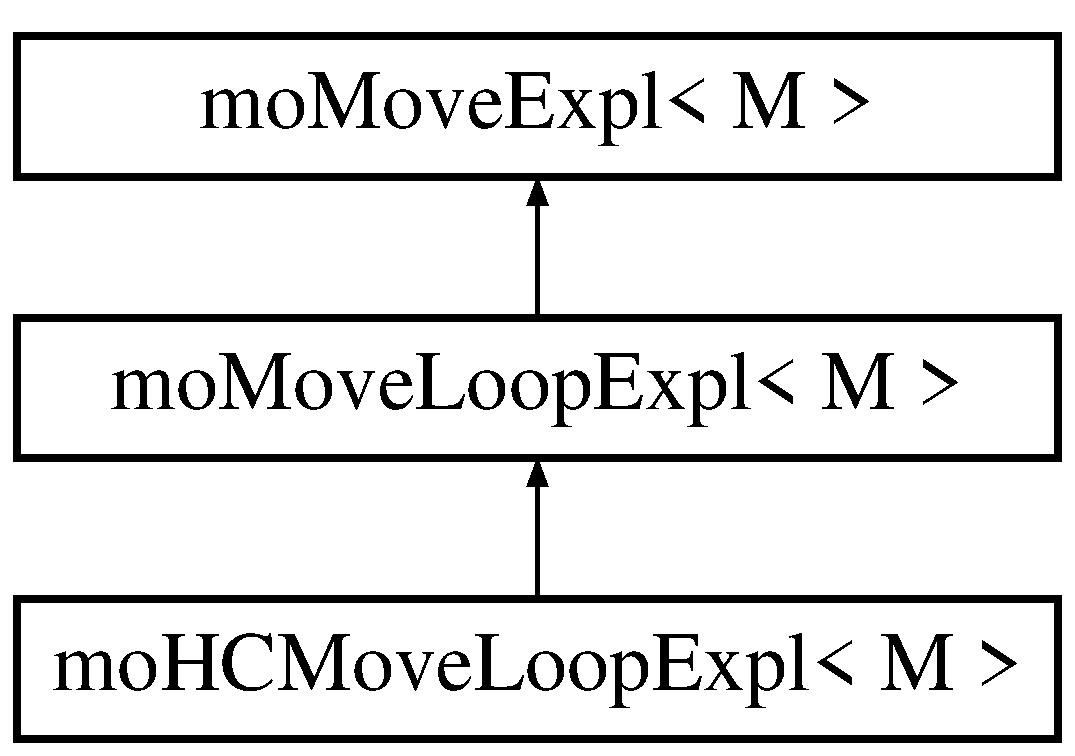
\includegraphics[height=5cm]{classmo_h_c_move_loop_expl}
\end{center}
\end{figure}
\subsection*{Public Member Functions}
\begin{CompactItemize}
\item 
{\bf mo\-HCMove\-Loop\-Expl} ({\bf mo\-Move\-Init}$<$ M $>$ \&\_\-move\_\-initializer, {\bf mo\-Next\-Move}$<$ M $>$ \&\_\-next\_\-move\_\-generator, {\bf mo\-Move\-Incr\-Eval}$<$ M $>$ \&\_\-incremental\_\-evaluation, {\bf mo\-Move\-Select}$<$ M $>$ \&\_\-move\_\-selection)
\begin{CompactList}\small\item\em Constructor. \item\end{CompactList}\item 
void {\bf operator()} (const {\bf EOT} \&\_\-old\_\-solution, {\bf EOT} \&\_\-new\_\-solution)
\begin{CompactList}\small\item\em Procedure which launches the explorer. \item\end{CompactList}\end{CompactItemize}
\subsection*{Private Types}
\begin{CompactItemize}
\item 
typedef M::EOType {\bf EOT}\label{classmo_h_c_move_loop_expl_y0}

\begin{CompactList}\small\item\em Alias for the type. \item\end{CompactList}\item 
typedef M::EOType::Fitness {\bf Fitness}\label{classmo_h_c_move_loop_expl_y1}

\begin{CompactList}\small\item\em Alias for the fitness. \item\end{CompactList}\end{CompactItemize}
\subsection*{Private Attributes}
\begin{CompactItemize}
\item 
{\bf mo\-Move\-Init}$<$ M $>$ \& {\bf move\_\-initializer}\label{classmo_h_c_move_loop_expl_r0}

\begin{CompactList}\small\item\em Move initialiser. \item\end{CompactList}\item 
{\bf mo\-Next\-Move}$<$ M $>$ \& {\bf next\_\-move\_\-generator}\label{classmo_h_c_move_loop_expl_r1}

\begin{CompactList}\small\item\em Neighborhood explorer. \item\end{CompactList}\item 
{\bf mo\-Move\-Incr\-Eval}$<$ M $>$ \& {\bf incremental\_\-evaluation}\label{classmo_h_c_move_loop_expl_r2}

\begin{CompactList}\small\item\em (generally) Efficient evaluation. \item\end{CompactList}\item 
{\bf mo\-Move\-Select}$<$ M $>$ \& {\bf move\_\-selection}\label{classmo_h_c_move_loop_expl_r3}

\begin{CompactList}\small\item\em Move selector. \item\end{CompactList}\end{CompactItemize}


\subsection{Detailed Description}
\subsubsection*{template$<$class M$>$ class mo\-HCMove\-Loop\-Expl$<$ M $>$}

Iterative explorer used by a {\bf mo\-HC}{\rm (p.\,\pageref{classmo_h_c})}. 



Definition at line 47 of file mo\-HCMove\-Loop\-Expl.h.

\subsection{Constructor \& Destructor Documentation}
\index{moHCMoveLoopExpl@{mo\-HCMove\-Loop\-Expl}!moHCMoveLoopExpl@{moHCMoveLoopExpl}}
\index{moHCMoveLoopExpl@{moHCMoveLoopExpl}!moHCMoveLoopExpl@{mo\-HCMove\-Loop\-Expl}}
\subsubsection{\setlength{\rightskip}{0pt plus 5cm}template$<$class M$>$ {\bf mo\-HCMove\-Loop\-Expl}$<$ M $>$::{\bf mo\-HCMove\-Loop\-Expl} ({\bf mo\-Move\-Init}$<$ M $>$ \& {\em \_\-move\_\-initializer}, {\bf mo\-Next\-Move}$<$ M $>$ \& {\em \_\-next\_\-move\_\-generator}, {\bf mo\-Move\-Incr\-Eval}$<$ M $>$ \& {\em \_\-incremental\_\-evaluation}, {\bf mo\-Move\-Select}$<$ M $>$ \& {\em \_\-move\_\-selection})\hspace{0.3cm}{\tt  [inline]}}\label{classmo_h_c_move_loop_expl_a0}


Constructor. 

All the boxes have to be specified.

\begin{Desc}
\item[Parameters:]
\begin{description}
\item[{\em \_\-move\_\-initializer}]The move initialiser. \item[{\em \_\-next\_\-move\_\-generator}]The neighbourhood explorer. \item[{\em \_\-incremental\_\-evaluation}](generally) Efficient evaluation function. \item[{\em \_\-move\_\-selection}]The move selector. \end{description}
\end{Desc}


Definition at line 66 of file mo\-HCMove\-Loop\-Expl.h.

References mo\-HCMove\-Loop\-Expl$<$ M $>$::incremental\_\-evaluation, mo\-HCMove\-Loop\-Expl$<$ M $>$::move\_\-initializer, mo\-HCMove\-Loop\-Expl$<$ M $>$::move\_\-selection, and mo\-HCMove\-Loop\-Expl$<$ M $>$::next\_\-move\_\-generator.

\subsection{Member Function Documentation}
\index{moHCMoveLoopExpl@{mo\-HCMove\-Loop\-Expl}!operator()@{operator()}}
\index{operator()@{operator()}!moHCMoveLoopExpl@{mo\-HCMove\-Loop\-Expl}}
\subsubsection{\setlength{\rightskip}{0pt plus 5cm}template$<$class M$>$ void {\bf mo\-HCMove\-Loop\-Expl}$<$ M $>$::operator() (const {\bf EOT} \& {\em \_\-old\_\-solution}, {\bf EOT} \& {\em \_\-new\_\-solution})\hspace{0.3cm}{\tt  [inline]}}\label{classmo_h_c_move_loop_expl_a1}


Procedure which launches the explorer. 

The exploration starts from an old solution and provides a new solution.

\begin{Desc}
\item[Parameters:]
\begin{description}
\item[{\em \_\-old\_\-solution}]The current solution. \item[{\em \_\-new\_\-solution}]The new solution (result of the procedure). \end{description}
\end{Desc}


Definition at line 79 of file mo\-HCMove\-Loop\-Expl.h.

References mo\-HCMove\-Loop\-Expl$<$ M $>$::Fitness, mo\-HCMove\-Loop\-Expl$<$ M $>$::incremental\_\-evaluation, mo\-HCMove\-Loop\-Expl$<$ M $>$::move\_\-initializer, mo\-HCMove\-Loop\-Expl$<$ M $>$::move\_\-selection, and mo\-HCMove\-Loop\-Expl$<$ M $>$::next\_\-move\_\-generator.

The documentation for this class was generated from the following file:\begin{CompactItemize}
\item 
mo\-HCMove\-Loop\-Expl.h\end{CompactItemize}
